%%%%%%%% ICML 2025 PAPER FILE %%%%%%%%%%%%%%%%%
%
% BUILD NOTE: this file needs icml2025.sty / icml2025.bst from the official
% ICML 2025 style bundle in the same directory. Figures are read from
% ../figures/ and ../outputs/, so compile from inside report/.
%
% Sections marked [TO BE COMPLETED] are placeholders for teammates.

\documentclass{article}

\usepackage{microtype}
\usepackage{booktabs}
\usepackage{amsmath}
\usepackage{amssymb}
\usepackage{graphicx}
\usepackage{multirow}
\usepackage{xcolor}

\usepackage{hyperref}
\usepackage[accepted]{icml2025}

\icmltitlerunning{Opinion Network Formation from Ordinal Questionnaire Data}

% ---- placeholder box for unfinished sections -------------------------------
\newcommand{\todoblock}[2]{%
  \vspace{0.4em}\noindent
  \fcolorbox{gray!60}{gray!10}{%
    \begin{minipage}{0.94\columnwidth}
      \footnotesize\textbf{[TO BE COMPLETED --- #1]}\\[0.2em]#2
    \end{minipage}}%
  \vspace{0.4em}
}

\begin{document}

\twocolumn[
\icmltitle{DPCN Assignment 1: Opinion Network Formation \\
from an Ordinal Attitude Questionnaire}

\begin{icmlauthorlist}
\icmlauthor{Arijeet Paul}{iiith}
\icmlauthor{Shreyash Lohare}{iiith}
\icmlauthor{Dev Patel}{iiith}
\end{icmlauthorlist}

\icmlaffiliation{iiith}{International Institute of Information Technology Hyderabad, India}
\icmlcorrespondingauthor{Arijeet Paul}{arijeet.paul@research.iiit.ac.in}

\icmlkeywords{network science, opinion dynamics, questionnaire analysis,
ordinal regression, missing data, Likert scale}

\vskip 0.2in
]

% Remove the next line if your copy of icml2025.sty does not define it.
\printAffiliationsAndNotice{}

\begin{abstract}
We construct and analyse an opinion network from a 60-item ordinal attitude
questionnaire answered by 96 respondents across four thematic blocks
(technology, education, society, environment). The work has three parts.
First, we sanitise the data while preserving the distinction between two
different missingness mechanisms: structural blanks left when a respondent
abandons the survey, and scattered ``No Comments'' (NC) responses inside
otherwise complete questionnaires. NC is not recoded as Neutral and NC users
are not discarded; missing responses are instead recovered by question-wise
regularised proportional-odds ordinal logistic regression, validated by
artificial masking under both missingness patterns. Second, we show that the
response distribution is severely ceilinged---$79.8\%$ of valid answers fall
on the agree side and the grand mean is $+1.14$ on a $[-2,+2]$ scale---so that
raw similarity measures how agreeable a respondent is rather than what they
believe. Row-centring each respondent removes this component and reduces the
number of item pairs correlated at $|r|\geq 0.30$ from $327$ to $42$. Third,
we build correlation networks over the sanitised matrix and run
Deffuant--Weisbuch bounded-confidence dynamics on a respondent network. We
show analytically and by controlled experiment that the widely reported
cluster plateau at small confidence thresholds is an arithmetic artefact of
the five-point response grid, while the difference between the sparse network
and a well-mixed population is a genuine effect of topology.
\end{abstract}

% ============================================================
\section{Introduction}
% ============================================================

Likert-scale questionnaires are a natural setting for studying how attitudes
in different domains relate to one another. Although each item is answered
independently, responses exhibit substantial dependence across questions and
across thematic domains. Network representations model these dependencies
directly: questionnaire items (or respondents) become vertices, and
statistical association becomes weighted edges.

Turning a questionnaire into a network is not, however, a mechanical step.
Three decisions determine whether the resulting graph carries signal or
merely re-describes the response format.

\textbf{How missing data is handled.} Missing responses arise both from
respondents stopping before reaching later questions and from respondents
declining to answer a particular item. These are different mechanisms
\cite{rubin1976inference} and should not be silently merged, and assigning a
numerical value such as Neutral to a declined answer injects information the
respondent never supplied.

\textbf{Whether response style is removed.} When respondents agree with almost
everything, correlation between any two items is inflated by a shared
``agreeableness'' component rather than genuine item association
\cite{paulhus1991measurement}. Unless this is removed, the network largely
encodes response style.

\textbf{What the network is compared against.} A correlation-derived network
has transitivity built into its construction, so clustering and modularity
appear even in structureless data. Any structural claim needs a null model
beside it.

This report addresses all three. Section~\ref{sec:data} documents the dataset
and its ceiling effect, Section~\ref{sec:handling} the sanitisation,
imputation and row-centring pipeline, Section~\ref{sec:analysis} the
individual analyses and visualisations, and
Sections~\ref{sec:discussion}--\ref{sec:conclusion} the findings and their
limits.

\paragraph{Team and code.}
Team \textbf{[TEAM NAME]}. All code, figures, and the data pipeline are
available at \url{https://github.com/shreyash-lohare/dpcn_a1_opinion_network}.
The full analysis is reproducible from a fresh clone via
\texttt{python run\_all.py} followed by the figure modules in \texttt{src/}.

% ============================================================
\section{Dataset Documentation}
\label{sec:data}
% ============================================================

The questionnaire contains 60 items in four thematic blocks of 15: technology
(T01--T15), education (E01--E15), society and ethics (S01--S15), and
environment (V01--V15). Each item offers five ordered categories plus an
explicit \emph{No Comments} option. For numerical analysis the categories are
encoded symmetrically,
\[
\text{SD}=-2,\quad \text{D}=-1,\quad \text{N}=0,\quad \text{A}=+1,\quad
\text{SA}=+2,
\]
which represents the ordering of the categories without asserting that
adjacent categories are equally spaced. Descriptive statistics in this section
are reported on the original $1$--$5$ scale (subtract $3$ to recover the
encoding above).

The raw file contains 96 respondent records and $96\times 60 = 5{,}760$ cells,
of which $5{,}255$ were answered and $5{,}218$ carry a substantive ordinal
response. Blocks are internally consistent to varying degrees: Cronbach's
$\alpha$ \cite{cronbach1951coefficient} is $0.87$ for environment and $0.82$
for society, but only $0.65$ for technology and $0.58$ for education, and
$0.885$ across all 60 items.

\subsection{The response ceiling}

The single most consequential property of this dataset is its ceiling.
Figure~\ref{fig:ceiling}(a) shows that $79.8\%$ of valid answers are
\emph{Agree} or \emph{Strongly Agree}, with \emph{Strongly Agree} alone
accounting for $43.1\%$; only $7.0\%$ of answers fall on the disagree side.
The grand mean is $4.138$ on the $1$--$5$ scale, i.e.\ $\mathbf{+1.14}$ on the
$[-2,+2]$ encoding.

Two consequences follow, and both shape every later decision. Item means
barely discriminate between statements, so the informative signal is in
\emph{which} statements attract disagreement rather than in overall agreement
level. And because almost every respondent agrees with almost everything, two
respondents will look similar under a raw similarity measure simply by both
being agreeable. Section~\ref{sec:centring} removes this component explicitly.

Figure~\ref{fig:ceiling}(b) shows the ceiling is not uniform across topics.
Environment ($\mu=4.39$, $89.5\%$ agree) and society ($\mu=4.28$, $86.0\%$)
are close to settled consensus, whereas technology ($\mu=3.99$, $8.1\%$
disagree) and especially education ($\mu=3.91$, $13.8\%$ disagree) retain
real disagreement. Notably, the blocks with the most disagreement are also
those with the lowest internal consistency, consistent with their items
tapping several distinct opinions rather than one settled disposition.

\begin{figure*}[t]
\centering
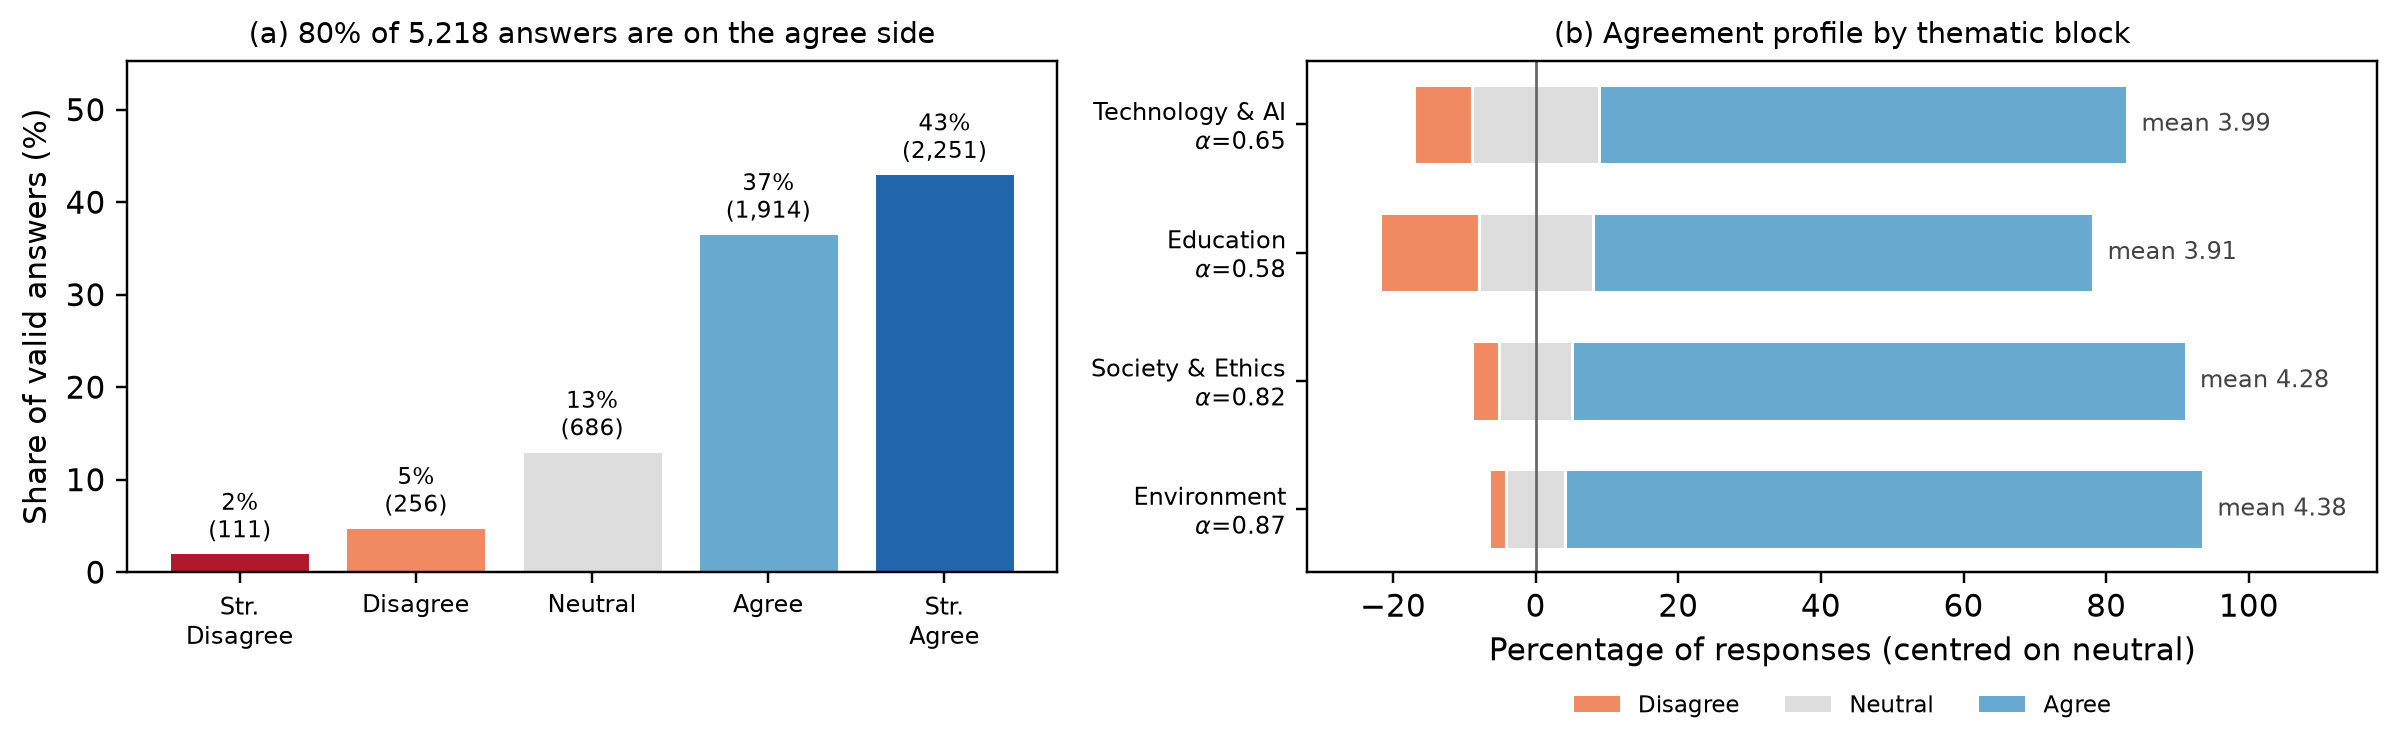
\includegraphics[width=0.88\textwidth]{../figures/fig_response_ceiling.png}
\caption{The response ceiling. (a) Distribution of all $5{,}218$ valid
answers: nearly four in five are on the agree side and $43\%$ are
\emph{Strongly Agree}. (b) Agreement profile per block, centred on neutral,
with block mean and Cronbach's $\alpha$. Environment and society are near
consensus; education carries the most disagreement and the weakest internal
consistency.}
\label{fig:ceiling}
\end{figure*}

\subsection{Where the disagreement lives}

Figure~\ref{fig:contested} ranks the twelve items attracting the most
disagreement. Seven are education items and four are technology items; only
one comes from society, and none from environment. Compulsory class attendance
(E03, mean $2.06$) is the only statement the cohort actively rejects, with
$70.1\%$ disagreeing and $40\%$ strongly disagreeing. Written examinations as
a measure of knowledge (E02, mean $2.84$) is the next most rejected.

The pattern is specific rather than generally oppositional: the same cohort
returns $94.3\%$ agreement that curricula should be updated more often (E11)
and that universities should prioritise problem-solving over rote learning
(E10). What is contested is assessment and teaching format, not the
institution.

The technology items behave similarly. Teaching AI (T04, $81.3\%$), AI as a
learning aid (T02, $79.1\%$), and AI accelerating research (T05, $81.3\%$) all
score high, whereas AI-assisted medical diagnosis (T08, mean $3.08$) and
autonomous vehicles (T09, mean $3.28$) are the two lowest technology items by
a clear margin. Since robots in hazardous occupations (T07) scores $82.4\%$
agreement, the objection is not to automation in general but to delegating
consequential judgment.

\begin{figure}[t]
\centering
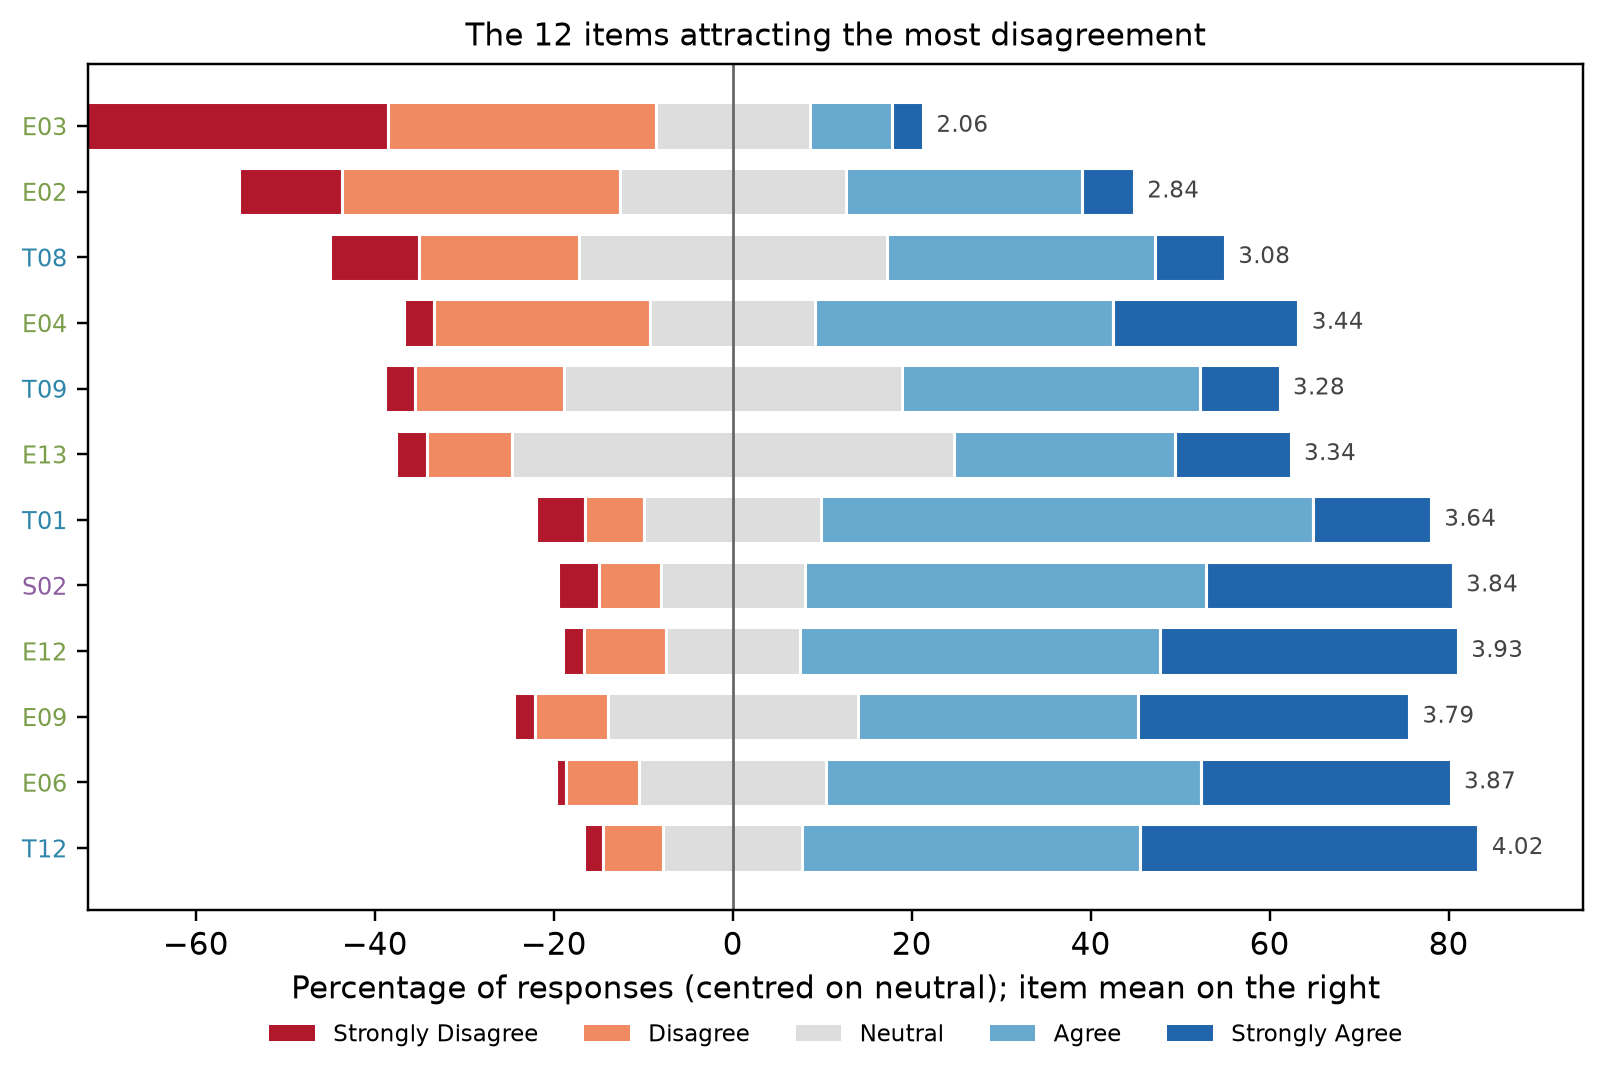
\includegraphics[width=0.92\columnwidth]{../figures/fig_contested_items.png}
\caption{The twelve items attracting the most disagreement, as diverging
response profiles centred on neutral, with item mean on the right. Labels are
coloured by block. Disagreement concentrates in education (7 of 12) and
technology (4 of 12).}
\label{fig:contested}
\end{figure}

\subsection{Missingness and data-quality notes}

Of the 96 records, 85 are complete, 5 are entirely empty, 4 stop after the
technology block, and 2 stop partway through environment. Dropout is therefore
\emph{monotone}---a truncated tail rather than scattered gaps---which matters
because it means later blocks rest on a slightly smaller base ($n=84$--$91$)
than earlier ones. Separately, 37 cells carry \emph{No Comments}, scattered
across 17 respondents who otherwise completed the questionnaire.

Three limitations should be carried into every result below. Items with means
above roughly $4.5$ measure social-desirability agreement more than strength
of preference. Only a small minority of statements are worded to invite
disagreement from an otherwise positive respondent, so acquiescence bias and
a genuine ceiling cannot be fully separated here. And the file contains no
demographic fields, so no finding can be attributed to a subgroup.

% ============================================================
\section{Data Handling}
\label{sec:handling}
% ============================================================

\subsection{Dataset sanitation}
\label{sec:sanitation}

\paragraph{Missingness structure.}
Five entirely empty records are excluded, leaving \textbf{91 respondents}. No
respondent is excluded for being merely incomplete: the four who stopped after
technology and the two who stopped during environment are retained, and their
unanswered items are treated as missing data to be recovered rather than as
grounds for deletion. This yields $205$ contiguous structural blank cells and
$37$ NC cells, $242$ missing cells in total among the retained respondents.

We distinguish
\[
\text{structural blank} = \text{question not reached},
\]
from
\[
\text{NC} = \text{deliberate non-response}.
\]
Both become missing values during modelling, but their original types are
retained so that preprocessing never silently conflates abandonment with an
explicit decision to withhold an answer.

\paragraph{Why NC is not Neutral.}
Recoding NC as Neutral would assign a substantive response to a cell for which
none was supplied. As a diagnostic we fitted a two-way additive model with
respondent and item effects on the clean responses,
$\hat{x}_{iq} = \bar{\mu} + a_i + b_q$. The fitted value at the 37 NC cells
averaged $3.92$ on the $1$--$5$ scale against $3$ for Neutral, so recoding
would impose a systematic downward shift of about $0.92$ scale points. This
model is used only as a diagnostic, not as the imputation method.

\paragraph{Empirical NC diagnostics.}
NC usage shows no systematic item- or respondent-level structure under the
tests applied. NC counts per item have a dispersion index of $1.10$ and a
chi-squared test of item-level uniformity gives $p=0.27$; no item carries more
than three NC responses; the correlation between NC frequency and item
standard deviation is $r=-0.02$. At respondent level, NC users have mean score
$4.01$ against $4.15$ for non-users ($p=0.27$), and neutral-response rates of
$0.123$ against $0.142$ ($p=0.82$). There is therefore no empirical basis for
assigning NC a fixed ordinal category, and we retain it as unobserved.

\paragraph{Sensitivity to NC treatment.}
Table~\ref{tab:sens} compares four NC treatments on the item-correlation
network at $\tau=0.30$. Dropping NC users would remove 17 respondents, roughly
a fifth of the sample, to eliminate only 37 cells, and it is the only
treatment that materially disturbs the recovered community structure
(AMI $0.337$). Correlations are far more stable than partitions across all
four treatments---a warning that stability of a correlation matrix should
never be read as evidence that a particular partition of it is stable.

\begin{table}[t]
\caption{Sensitivity of the item-correlation network to NC treatment at
$\tau=0.30$, against pairwise deletion as reference. Computed at an earlier
86-respondent configuration; ordering of the treatments is the result of
interest rather than the absolute counts.}
\label{tab:sens}
\vskip 0.05in
\begin{center}
\footnotesize
\begin{tabular}{lrrrrr}
\toprule
Treatment & $N$ & $E$ & $r$ & Jacc. & AMI \\
\midrule
Pairwise delete (ref.) & 86 & 325 & -- & -- & -- \\
Recode $\rightarrow$ Neutral & 86 & 333 & .993 & .875 & .662 \\
Drop NC users & 69 & 362 & .947 & .616 & .337 \\
Two-way impute & 86 & 335 & .997 & .924 & .670 \\
\bottomrule
\end{tabular}
\end{center}
\vskip -0.1in
\end{table}

\subsection{Missing-value imputation}
\label{sec:imputation}

\paragraph{Ordinal regression formulation.}
For target item $j$ the remaining 59 items form the predictor vector
$\mathbf{x}_{i,-j}$, and the target satisfies
$y_{ij}\in\{-2,-1,0,+1,+2\}$. We fit one regularised proportional-odds ordinal
logistic regression \cite{mccullagh1980regression} per item, with latent score
$z_i = \beta_0 + \boldsymbol{\beta}^{\top}\mathbf{x}_{i,-j}$ and ordered
thresholds $\theta_1<\theta_2<\theta_3<\theta_4$ inducing the five response
intervals. The prediction is the maximum-probability category,
\[
\hat{y}_{ij} = \arg\max_k P(y_{ij}=k \mid \mathbf{x}_{i,-j}).
\]
This preserves the ordering of the Likert responses while avoiding the
interval-scale assumption of linear regression, and unlike nominal multiclass
classification it retains the relative order of the five outcomes.

\paragraph{Missing predictors and regularisation.}
A respondent may have several missing cells, so predictors that are themselves
missing cannot be encoded as Neutral. They are instead filled with the
training-fold column median before standardisation, with the statistic
computed only from training data in each fold to prevent leakage from held-out
responses. A ridge penalty controls complexity in the 59-dimensional predictor
space, and the target is always excluded from its own predictor vector, giving
$M_j:\mathbf{X}_{-j}\rightarrow Y_j$ for $j=1,\ldots,60$.

\paragraph{Validation.}
The true values of the $242$ genuinely missing cells are unavailable, so the
pipeline is evaluated by artificial masking of responses whose values are
known, under two mechanisms matched to the two missingness types.
\emph{Scattered masking} hides 37 observed cells at random inside otherwise
complete respondents, approximating NC, over 40 trials. \emph{Suffix masking}
hides a contiguous tail after a simulated stopping point drawn from the
observed stopping pattern, for 15 respondents per trial over 15 trials; items
after the stopping point are withheld from the predictor so the model cannot
use information unavailable in practice.

\begin{table}[t]
\caption{Artificial-masking validation. Accuracy is exact-category; MAE is
mean absolute error on the five-point scale.}
\label{tab:val}
\vskip 0.05in
\begin{center}
\footnotesize
\begin{tabular}{lcccc}
\toprule
& \multicolumn{2}{c}{Ordinal model}
& \multicolumn{2}{c}{Mode baseline} \\
Masking & Acc. & MAE & Acc. & MAE \\
\midrule
Scattered (NC-like) & .539 & .534 & .486 & .626 \\
Suffix (structural) & .498 & .612 & .482 & .655 \\
\bottomrule
\end{tabular}
\end{center}
\vskip -0.1in
\end{table}

Because the target is ordinal, MAE is the more informative metric: a
prediction one category away is not the same error as one at the opposite end
of the scale. Table~\ref{tab:val} shows the model beats a modal-response
baseline under both mechanisms, by a wider margin under scattered masking
where more co-answered items remain available. Performance is lower under
suffix masking precisely because fewer predictors survive the stopping point,
so the two settings should be read separately rather than averaged into one
number. The final model imputes all $242$ missing cells, with every recovered
value restricted to the original five-level support.

\subsection{Row-centring}
\label{sec:centring}

Imputation yields a complete $91\times 60$ matrix on the original scale, but
not one that can be correlated directly. Because the grand mean is $+1.14$
(Section~\ref{sec:data}), a respondent who agrees with everything raises all
60 of their entries together, which appears as association between every pair
of items at once. We therefore replace each entry by its deviation from that
respondent's own mean,
\begin{equation}
x'_{i,j} = x_{i,j} - \bar{x}_{i\cdot},
\qquad
\bar{x}_{i\cdot} = \frac{1}{60}\sum_{k=1}^{60} x_{i,k}.
\end{equation}

Two points are worth stating precisely. First, centring is applied strictly
\emph{after} imputation and strictly \emph{before} correlation: the imputation
model predicts on the original $-2$ to $+2$ scale, and centring is a
network-construction step, not a data-cleaning one. Second, rank correlation
does not remove this bias automatically---Spearman correlation is invariant to
a monotone transform of a single column, not to an additive shift that differs
from row to row. The magnitude of the effect is reported as Graph~3
(Section~\ref{sec:g3}).

\subsection{Network construction}

On the sanitised, row-centred matrix we build a weighted undirected graph
$G=(V,E,W)$ whose 60 vertices are the questionnaire items. Because responses
are ordered categories, the primary association measure is the Spearman rank
correlation $\rho_{qr}$, and edge weights are signed correlations, with
$|\rho_{qr}|$ used for edge magnitude in visualisation and sign distinguished
by colour. We retain the full weighted matrix and threshold only for display,
showing an edge when $|\rho_{qr}| \geq \tau$. The association step is
implemented modularly so a latent-variable ordinal measure such as polychoric
correlation can replace Spearman without changing graph construction. A second,
\emph{respondent}-level network is introduced in Section~\ref{sec:g12} for the
dynamics experiment.

% ============================================================
\section{Analysis and Visualisations}
\label{sec:analysis}
% ============================================================

This section reports the twelve analyses. Each states what the figure shows,
what was found, and what follows from it. Sections still owned by other team
members are marked as placeholders.

\paragraph{A note on respondent counts.}
Several reference values circulated during planning assume a pipeline variant
that drops respondents with more than 12 missing items, leaving 86. This
report does \emph{not} use that filter: all 91 non-empty respondents are
retained and their missing cells recovered by ordinal regression
(Section~\ref{sec:imputation}). Figures produced here therefore report
$n=91$, and small deviations from those reference numbers are expected.

\subsection{Graph 1: Missingness map and response distribution}
\label{sec:g1}

Figure~\ref{fig:g1} shows every cell of the raw $96\times 60$ matrix as
missing or present, with respondents sorted by missing count, beside the
distribution of per-respondent mean scores.

\textbf{Findings.} The $542$ missing cells ($505$ structural blanks plus $37$
NC) are extremely unevenly distributed. Five respondents are entirely empty
and account for $300$ of them; the remaining $242$ are spread thinly across
the other 91, a missing rate of $4.4\%$. Below the cutoff the map is almost
clean, with scattered single cells and two visible tails from the respondents
who stopped early. The right panel locates the grand mean at $1.14$, with the
bulk of respondents between $0.75$ and $1.50$ and only one respondent below
zero.

\textbf{Implication.} The missingness structure justifies the retention policy
directly. Because all but five respondents answered at least $80\%$ of items,
there is no population of badly-incomplete respondents whose removal would
simplify the analysis, and a count-based exclusion rule would discard usable
respondents to remove very few cells. The right panel is the first direct
evidence of the acquiescence problem that Section~\ref{sec:centring} corrects.

\begin{figure*}[t]
\centering
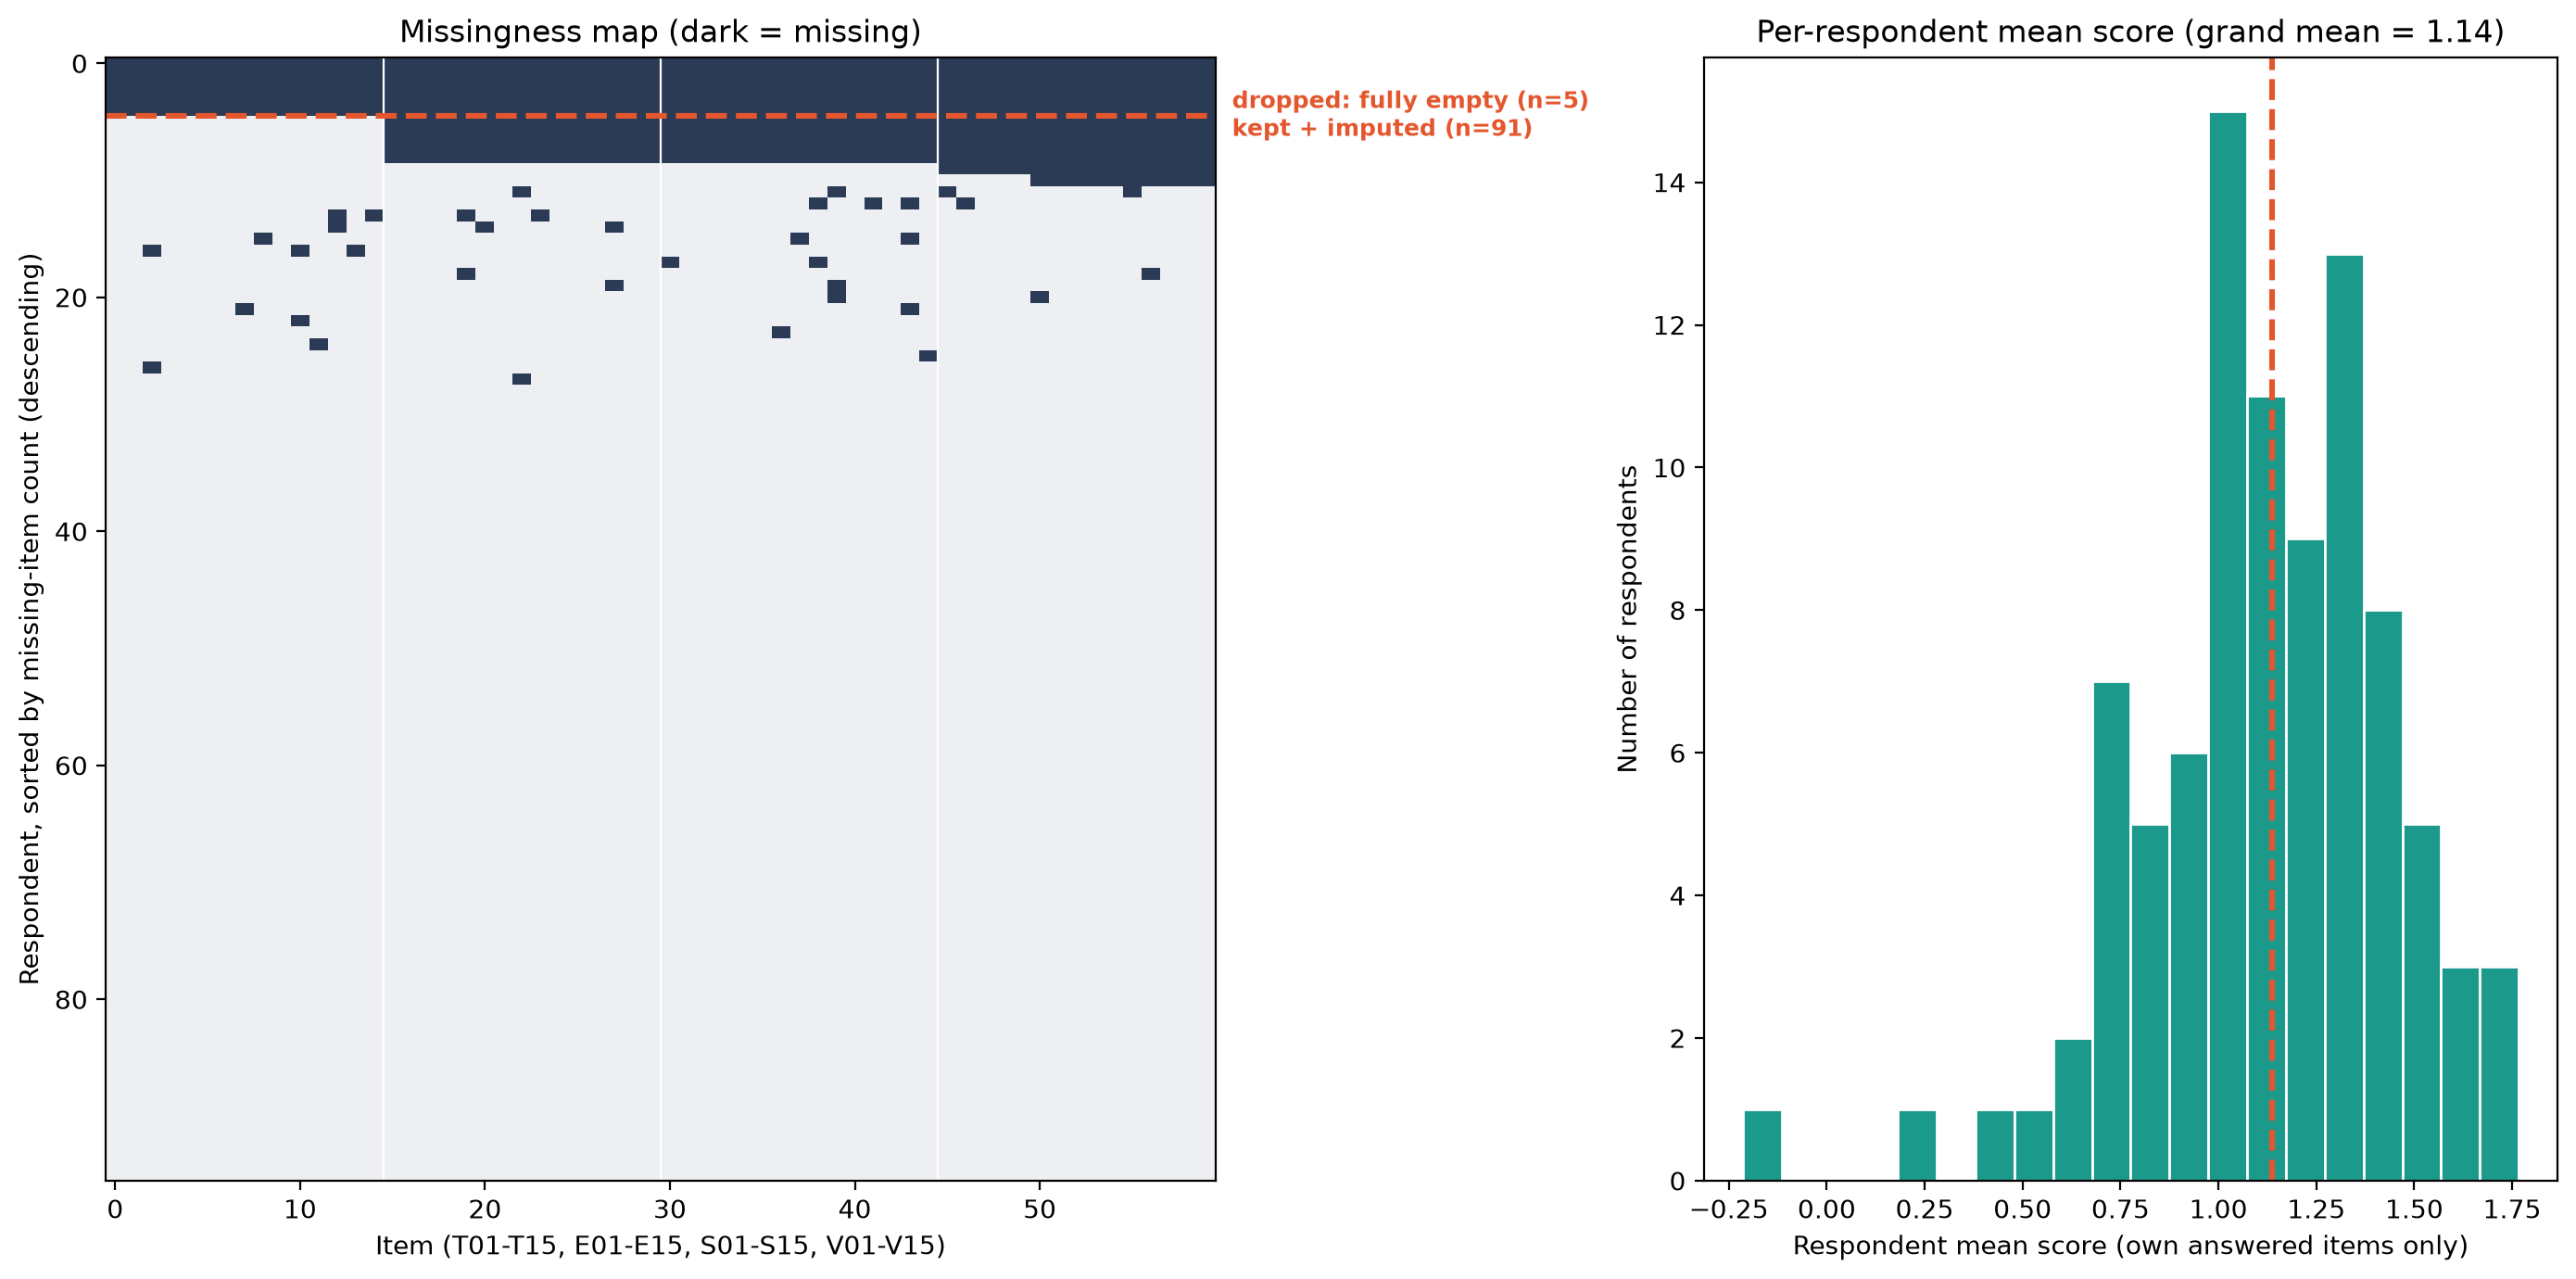
\includegraphics[width=0.86\textwidth]{../figures/graph1_missingness_response_distribution.png}
\caption{Graph 1. Left: missingness map over all 96 raw respondents, sorted by
missing-item count; dark cells are missing for either reason. The dashed line
marks this project's exclusion rule---only the five entirely empty records are
dropped, and the remaining 91 respondents have their $242$ missing cells
imputed. Right: per-respondent mean over answered items only, with the grand
mean at $1.14$.}
\label{fig:g1}
\end{figure*}

\subsection{Graph 2: Item variance ranking}
\label{sec:g2}

Figure~\ref{fig:g2} ranks all 60 items by standard deviation on the
\emph{uncentred} imputed matrix. Centring is deliberately not applied here: it
changes each item's variance and would answer a different question (spread
after removing each respondent's baseline) than the one asked (how divided the
cohort is on the statement as posed).

\textbf{Findings.} Item SD ranges from $0.50$ (E15, ``continuous learning is
essential'', near-unanimous) to $1.18$ (E04, online learning). The five most
contested items are E04, E03, E02, T08 and T07; the least contested include
V13, V06, S05 and E15. By block mean SD the order is technology $0.92$,
education $0.88$, society $0.79$, environment $0.72$.

\textbf{Implication.} The block averages and the extremes tell slightly
different stories, and both matter. Technology has the highest average
variance, but the \emph{sharpest} disagreements are educational: three of the
five most divided items are E02--E04, all concerning assessment and teaching
format. Environment contributes none of the top ten. This is a property of the
survey instrument, not of preprocessing: the questionnaire contains a settled
domain (environment), a moderately settled one (society), and two live ones
(technology, education). Consensus items carry little information for a
correlation network---an item everyone endorses cannot covary with anything---
so the network's signal is necessarily concentrated in the contested tail.

\begin{figure}[t]
\centering
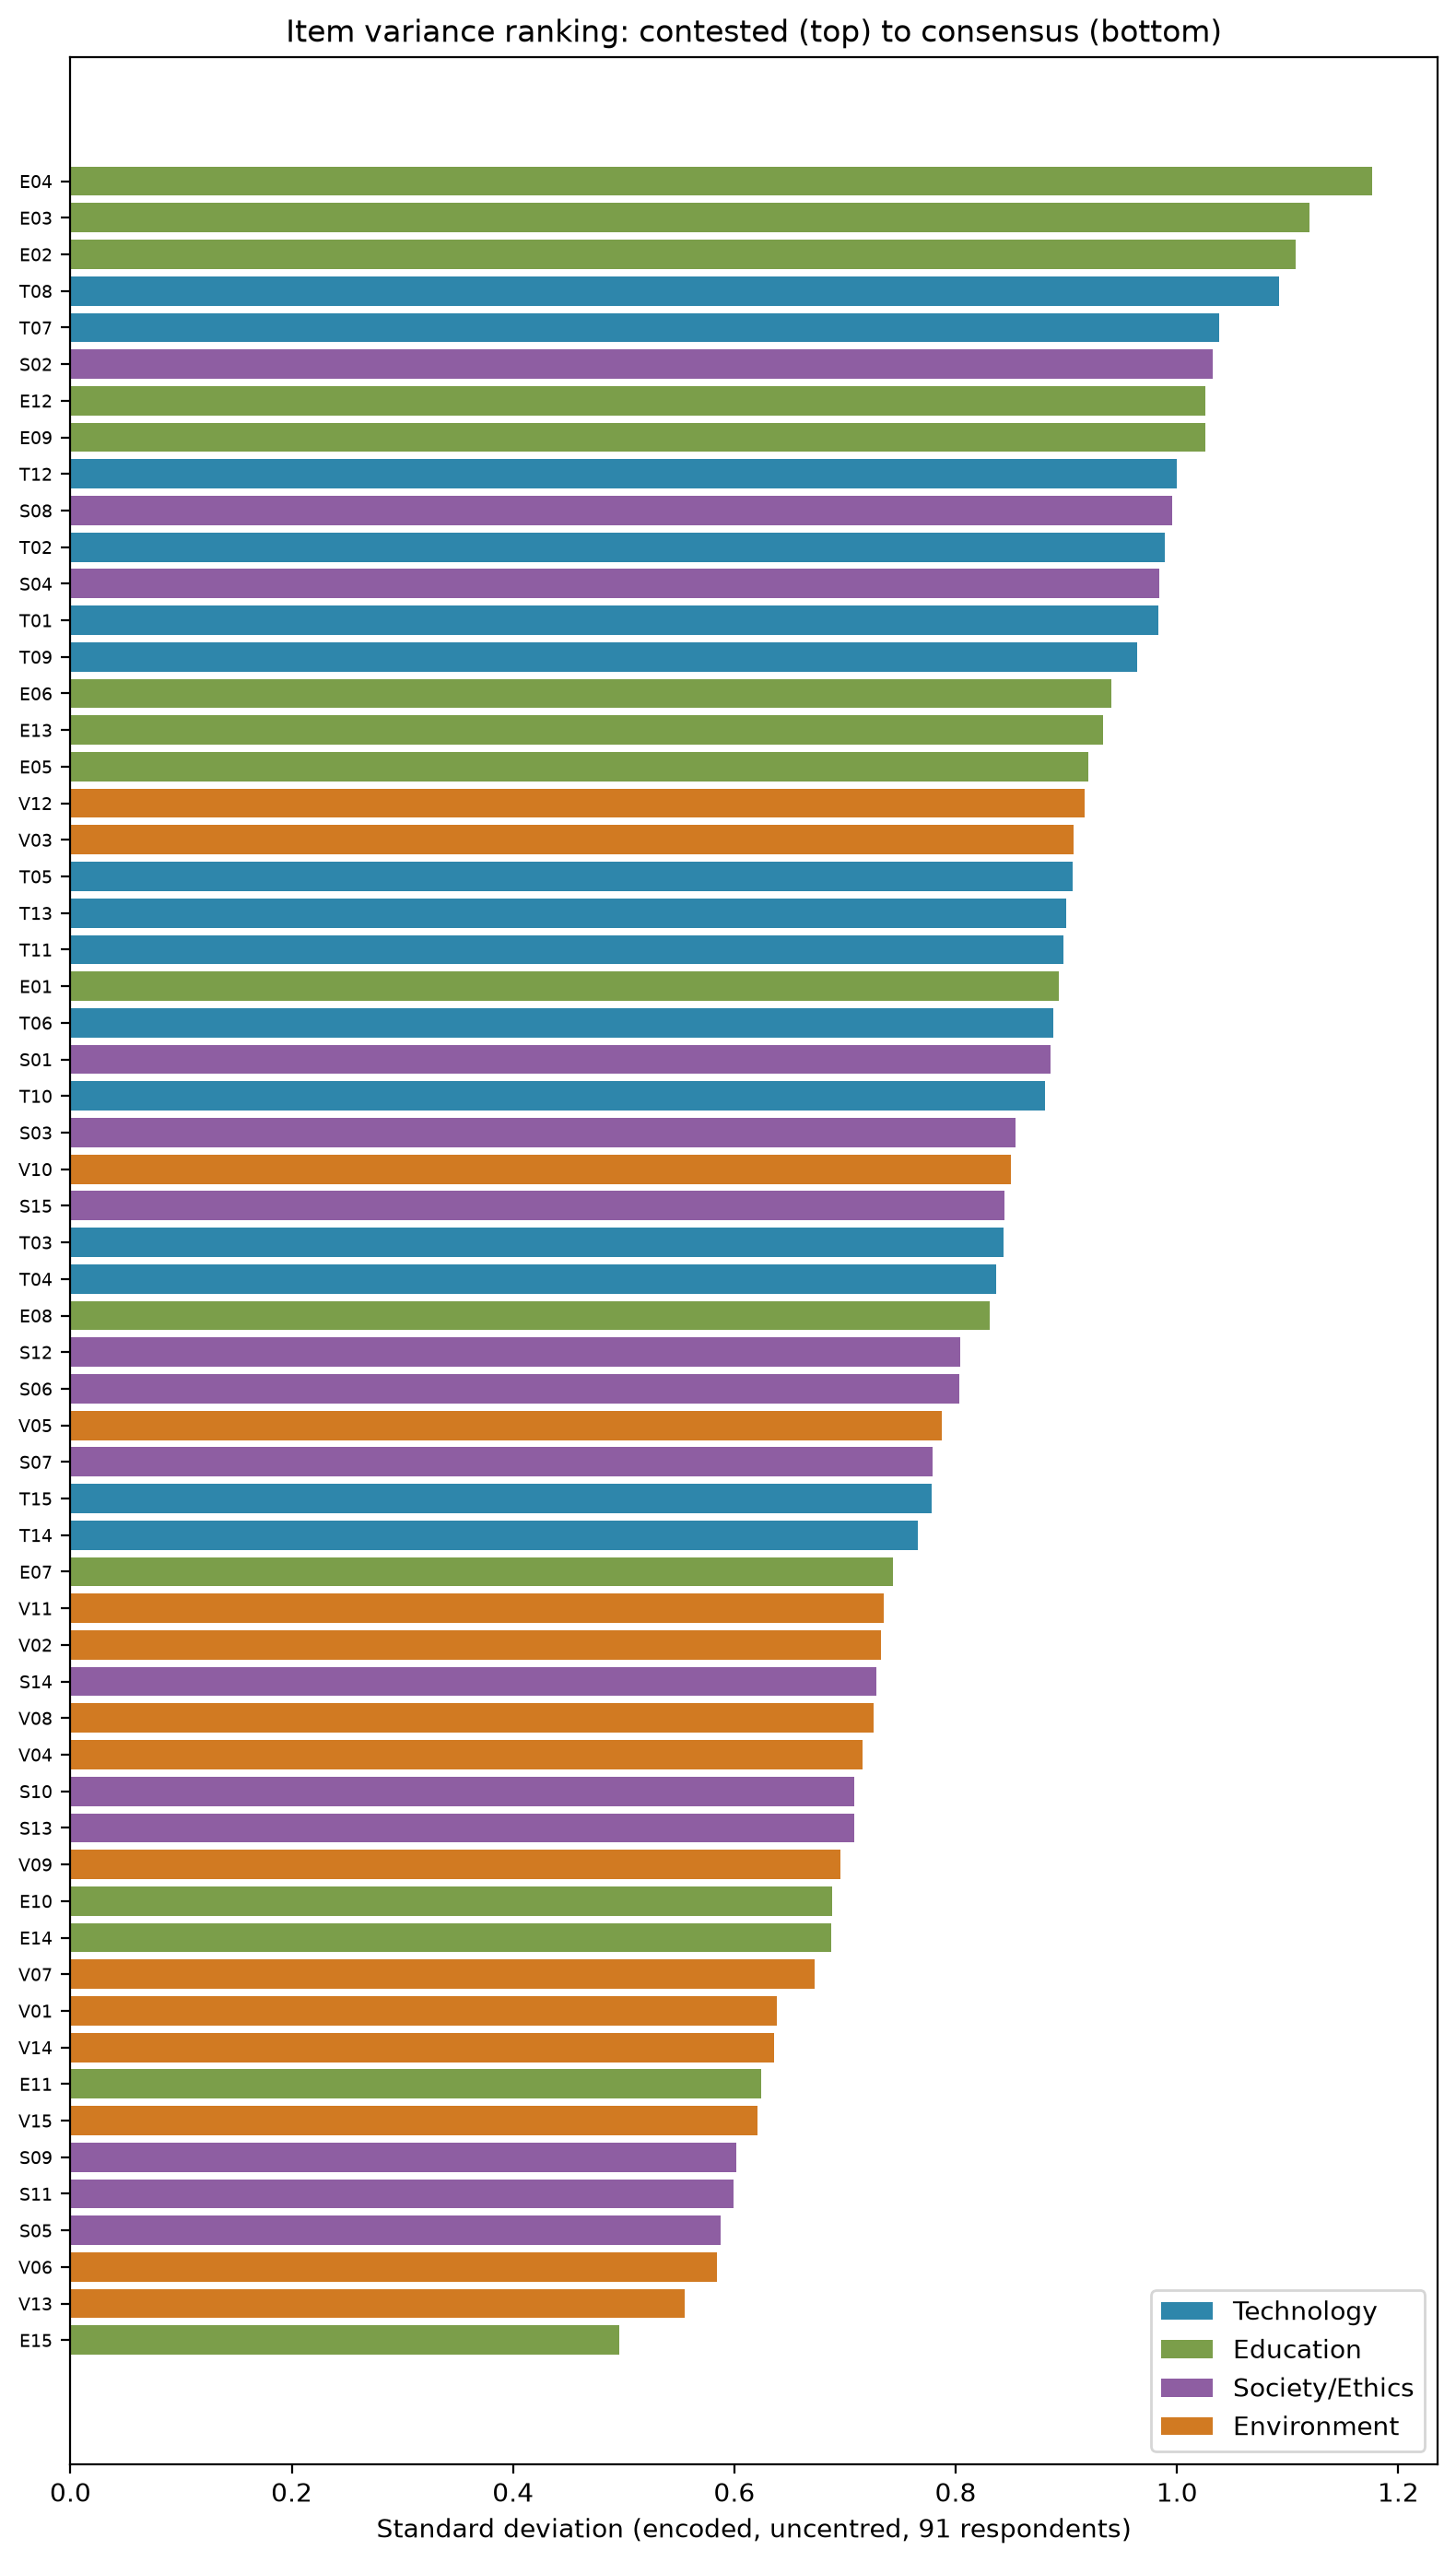
\includegraphics[width=0.66\columnwidth]{../figures/graph2_item_variance_ranking.png}
\caption{Graph 2. All 60 items ranked by standard deviation on the uncentred
imputed matrix, coloured by block. Contested items (top) concentrate in
education and technology; environment items cluster at the consensus end.}
\label{fig:g2}
\end{figure}

\subsection{Graph 3: The effect of row-centring}
\label{sec:g3}

Figure~\ref{fig:g3} overlays the distribution of all
$\binom{60}{2}=1{,}770$ pairwise item correlations computed before and after
row-centring, on identical bin edges.

\textbf{Findings.} The raw distribution is displaced positive, with mean
$r=0.151$ and median $0.151$; almost no pair is appreciably negative. After
centring the distribution sits essentially on zero, mean $r=-0.004$, median
$-0.008$, with positive skew ($0.221$) leaving a heavier right tail of
genuinely co-varying pairs. At a fixed threshold of $|r|\geq 0.30$ the number
of surviving pairs falls from $\mathbf{327}$ to $\mathbf{42}$, a reduction of
$87\%$.

\textbf{Implication.} This converts the claim of Section~\ref{sec:centring}
from an assertion into a measurement: roughly seven eighths of the apparent
association in the raw matrix is shared response style, not item
relationship. Had the network been built on raw scores it would have been
dense, almost entirely positive, and would have supported confident but
spurious conclusions about item structure. The surviving $42$ pairs are the
only ones worth interpreting, and the emergence of negative correlations after
centring---impossible to see in the raw distribution---is what later permits a
signed-network analysis at all.

\begin{figure}[t]
\centering
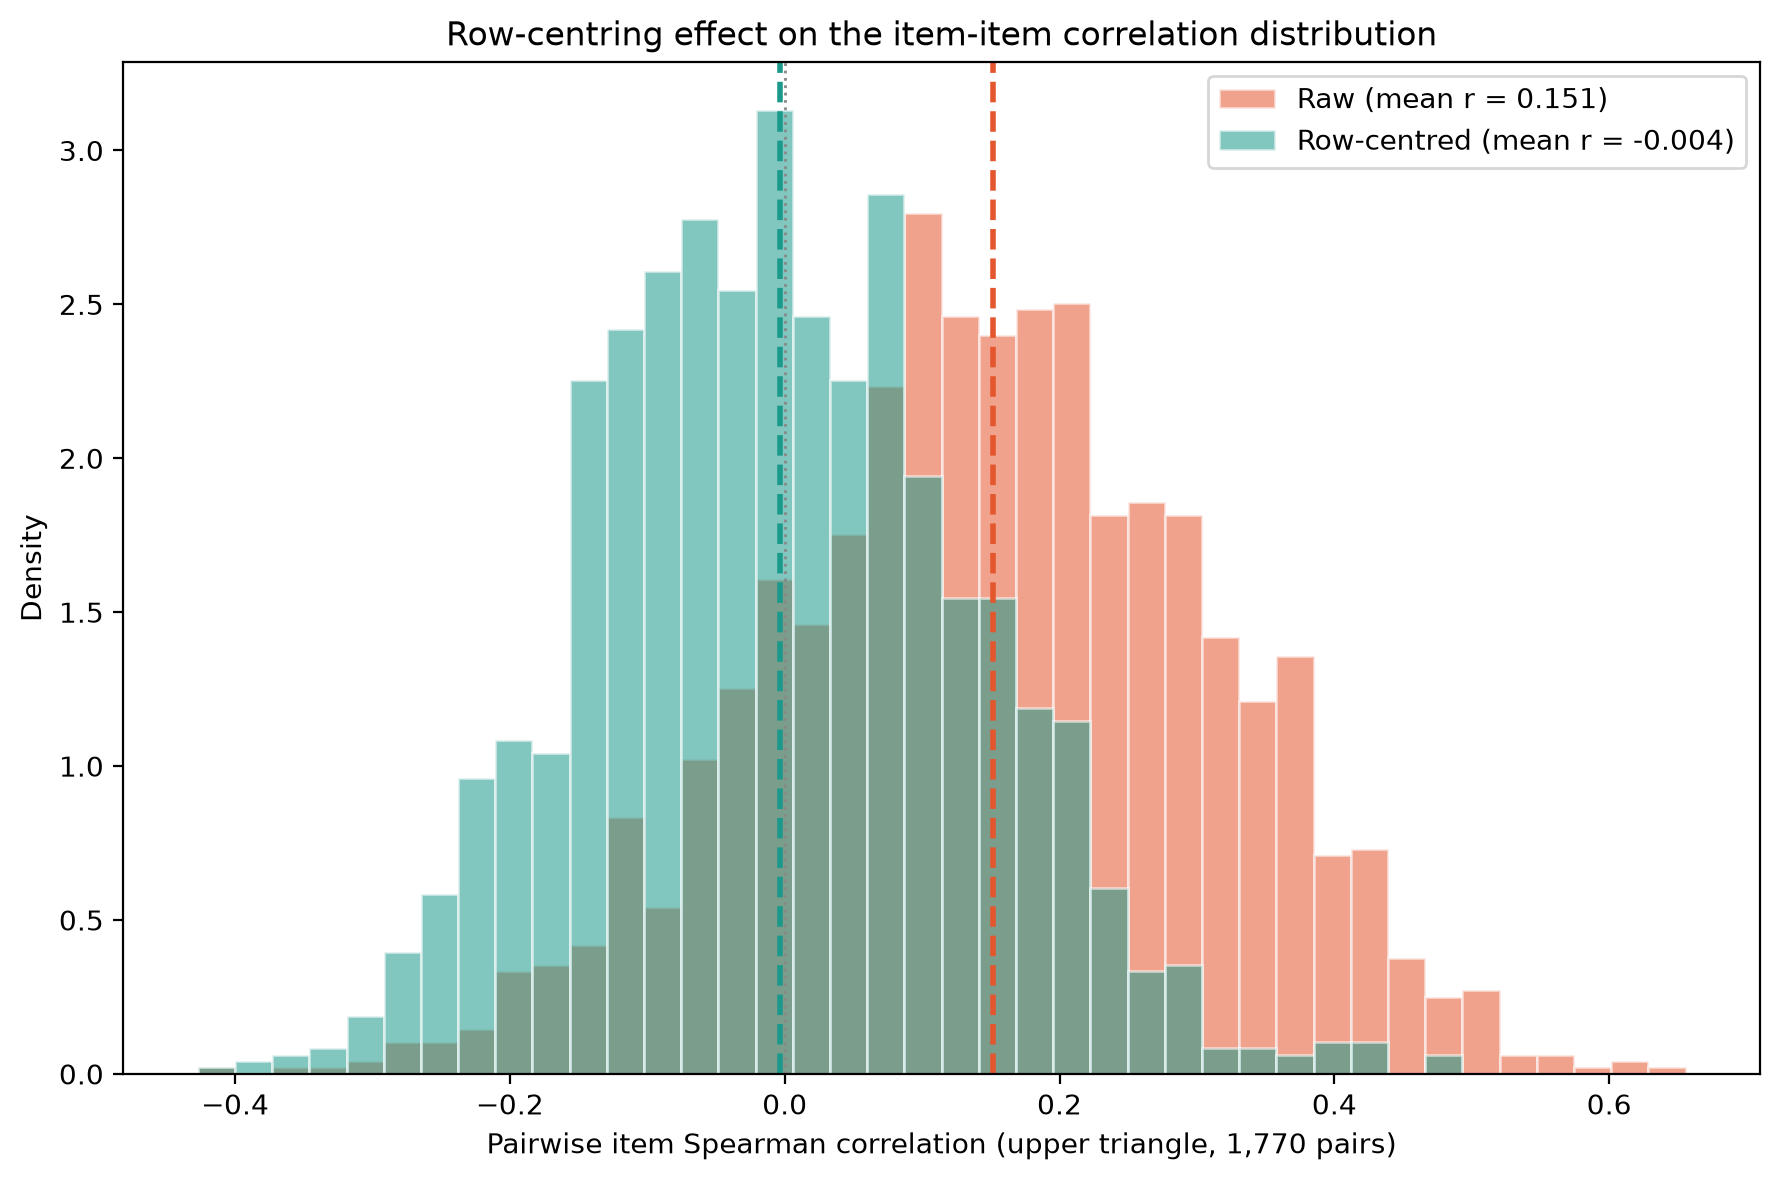
\includegraphics[width=0.94\columnwidth]{../figures/graph3_row_centring_effect.png}
\caption{Graph 3. Distribution of all $1{,}770$ pairwise item correlations
before and after row-centring, on shared bin edges. Centring moves the mean
from $0.151$ to $-0.004$ and removes $87\%$ of the pairs exceeding
$|r|\geq0.30$.}
\label{fig:g3}
\end{figure}

\subsection{Graph 4: Real versus shuffled correlations}

\todoblock{Graph 4 --- owner: P2}{%
Compare the distribution of observed item--item correlations against a
column-shuffled null that destroys inter-item structure while preserving each
item's marginal. Plot both distributions and report the excess of real edges
over chance at several thresholds.\\[0.25em]
\emph{Reference values to check against:} real SD $0.136$ vs shuffled SD
$0.108$ (theoretical $1/\sqrt{n-3}\approx0.109$); edges at $|r|>0.15$: $467$
real vs $309$ chance; $>0.20$: $258$ vs $118$; $>0.25$: $111$ vs $37$;
$>0.30$: $49$ vs $9$.\\[0.25em]
\emph{Findings + implication:} to be written.}

\subsection{Graph 5: Eigenvalue spectrum against Marchenko--Pastur}

\todoblock{Graph 5 --- owner: P2}{%
Plot the eigenvalue spectrum of the row-centred correlation matrix against the
Marchenko--Pastur band \cite{marchenko1967distribution} for a random matrix of
the same shape, to separate informative modes from noise.\\[0.25em]
\emph{Reference values:} with $T$ respondents and $N=60$ items, $Q=T/N$ and
$\lambda_+=(1+1/\sqrt{Q})^2$. At $T=86$ this gives $\lambda_+\approx3.368$,
with exactly three eigenvalues above it ($4.05$, $3.98$, $3.53$) carrying
$19.3\%$ of total variance. Recompute for $T=91$.\\[0.25em]
\emph{Findings + implication:} to be written. Note that PC1 explains only
about $8\%$ of variance, so this should \emph{not} be read as evidence of a
two-camp polarisation.}

\subsection{Graph 6: Reordered correlation heatmap}

\todoblock{Graph 6 --- owner: P3}{%
Correlation matrix with rows and columns reordered by detected community so
that communities appear as diagonal blocks, with a colour scale that
distinguishes sign.\\[0.25em]
\emph{Findings + implication:} to be written. State explicitly whether the
diagonal blocks align with the four thematic blocks or cut across them ---
that comparison is the point of the figure.}

\subsection{Graph 7: Threshold and percolation sweep}

\todoblock{Graph 7 --- owner: P2}{%
Sweep the edge threshold $\tau$ and plot number of connected components,
modularity, and average clustering against it, to select $\tau$ by evidence
rather than convention. This figure supplies the threshold used by Graph 8.
\\[0.25em]
\emph{Findings + implication:} to be written. Report the chosen $\tau$ and the
justification, and note the trade-off between a connected graph and one whose
edges are individually trustworthy.}

\subsection{Graph 8: Main item network}

\todoblock{Graph 8 --- owner: P1, blocked on Graph 7}{%
The item--item network at the threshold selected in Graph 7, nodes coloured by
thematic block, edges signed and weighted by correlation magnitude.\\[0.25em]
\emph{Dependency:} the threshold must come from the Graph 7 sweep rather than
being chosen here.\\[0.25em]
\emph{Findings + implication:} to be written. Report the number of connected
items and isolates at the chosen threshold, which items act as hubs, and
whether edges respect block boundaries.}

\subsection{Graph 9: Topic-block connectivity}

\todoblock{Graph 9 --- owner: P1}{%
$4\times4$ heatmap of connectivity between the four thematic blocks,
summarising how strongly each pair of topics is linked.\\[0.25em]
\emph{Reference values (respondent-level block-score correlations):} T--E
$0.29$, T--S $0.54$, T--V $0.46$, E--S $0.53$, E--V $0.49$, S--V $\mathbf{0.70}$.
The raw values are available in \texttt{data/uc\_survey\_derived.json}.
\\[0.25em]
\emph{Findings + implication:} to be written. The headline is that society and
environment behave as a single ``civic and ecological responsibility''
disposition, while technology and education are close to independent
($r=0.29$, the weakest pair) --- views on AI and views on pedagogy are
separate axes.}

\subsection{Graph 10: Communities against null models}

\todoblock{Graph 10 --- owner: P3}{%
Compare observed modularity and clustering against three nulls: a
degree-preserving rewiring \cite{maslov2002specificity}, an
Erd\H{o}s--R\'enyi graph, and a column-permutation null that regenerates the
entire pipeline from scrambled responses.\\[0.25em]
\emph{Reference values (respondent network):} modularity $0.408$--$0.423$ and
clustering $0.202$ observed; rewiring null $0.329\pm0.011$ ($z\approx7$) and
$0.091\pm0.013$ ($z\approx8.9$), both passed; permutation null
$0.403\pm0.017$ ($z\approx1.15$), \textbf{not} passed.\\[0.25em]
\emph{Findings + implication:} to be written. The permutation null is the
decisive one: rewiring and ER take the finished graph as given and cannot
detect transitivity introduced by the correlation-and-threshold construction
itself. If modularity clears rewiring but not permutation, the community
structure is largely a construction artefact and must be reported as such ---
this is a finding, not a failure.}

\subsection{Graph 11: Structural balance}

\todoblock{Graph 11 --- owner: P3}{%
Fraction of balanced triads in the signed item network as a function of
threshold, against a sign-permutation null
\cite{cartwright1956structural}.\\[0.25em]
\emph{Reference values:} balanced-triad fraction $83\%$ at $|r|>0.15$, $96\%$
at $0.20$, $100\%$ at $0.25$, against roughly $50\%$ under the null.\\[0.25em]
\emph{Findings + implication:} to be written. That the fraction strengthens as
the threshold tightens is itself part of the evidence, since a spurious effect
would not sharpen as weak edges are removed.}

\subsection{Graph 12: Opinion dynamics}
\label{sec:g12}

This is the only analysis involving an actual dynamical process; everything
above describes a fixed dataset. Because each opinion is one respondent's
answer to one item, the vertices here are \emph{respondents}, not items, so a
second network is required.

\paragraph{The respondent network.}
From the row-centred matrix we compute the $91\times91$ Pearson correlation
between respondents and connect each respondent to their $k=4$ most similar
peers, symmetrising by union. Union rather than mutual $k$NN is deliberate:
mutual $k$NN fragments this data badly, and disconnected components cannot
merge at any confidence threshold, which would inflate the final cluster count
for reasons unrelated to the dynamics. The result has $91$ nodes, $298$ edges,
mean degree $6.55$, and forms a \emph{single connected component}.

\paragraph{The model.}
Opinions $x_i\in[0,1]$ are seeded from item E03 (compulsory attendance, SD
$1.12$), rescaled by $s(x)=(x+2)/4$. At each step a random edge $(u,v)$ is
drawn, and if the two opinions lie within the confidence threshold they move
to their midpoint \cite{deffuant2000mixing}:
\begin{equation}
|x_u - x_v| < \varepsilon
\ \Longrightarrow\
x_u,x_v \leftarrow \tfrac{1}{2}\left(x_u + x_v\right).
\end{equation}
We sweep $\varepsilon$ from $0.05$ to $0.60$ in steps of $0.05$, with 20
seeded repetitions of up to $60{,}000$ interactions each, terminating early on
convergence, and count final clusters by rounding to two decimals.

\paragraph{Findings.}
Results appear in Figure~\ref{fig:g12} and Table~\ref{tab:dw}. Cluster count
is exactly $5.00\pm0.00$ for every $\varepsilon\leq0.25$, then falls to $4.45$
at $\varepsilon=0.30$, $3.35$ at $0.40$, $2.00$ at $0.50$, approaching
consensus near $0.55$--$0.60$.

\paragraph{The plateau is an artefact, and provably so.}
The specification for this analysis requires stating that the low-$\varepsilon$
plateau is partly an artefact of the discrete five-point grid. In fact the
claim can be made exactly. Under $s(x)=(x+2)/4$ the five categories map to
$\{0,\tfrac14,\tfrac12,\tfrac34,1\}$, so any two distinct initial opinions
differ by at least $\tfrac14$. For any $\varepsilon\leq0.25$ the condition
$|x_u-x_v|<\varepsilon$ is therefore \emph{never} satisfied by a pair with
distinct opinions: the initial state is a fixed point and the final count
equals the number of occupied categories, on any graph whatsoever.

Three observations confirm this empirically. The plateau has \emph{zero}
variance across 20 randomly seeded runs, which no genuine emergent outcome
would. A complete graph---a maximally different topology---returns the
identical $5.00\pm0.00$ over the same range. And re-running with seeds
jittered by $\pm0.125$, which destroys the grid while preserving the
distribution's shape, removes the plateau entirely, yielding
$35.95\rightarrow26.35\rightarrow21.05\rightarrow14.20\rightarrow8.95$
clusters across $\varepsilon=0.05\ldots0.25$. The five clusters below
$\varepsilon=0.25$ are the original response categories failing to merge, not
opinion groups forming, and the break in the curve at $\varepsilon=0.30$ is
arithmetic rather than a discovered threshold.

\paragraph{What is not an artefact.}
The substantive result lies above $\varepsilon=0.25$. Comparing the real
network against an identically seeded complete graph---the same dynamics with
topology removed---the well-mixed population collapses to about $2$ clusters
across $\varepsilon=0.30$--$0.45$, while the sparse $k$NN network sustains
$3.15$--$4.45$. Network structure therefore \emph{sustains opinion diversity
that a well-mixed population loses at the same tolerance}: when respondents
interact only with their nearest neighbours in opinion space, locally cohesive
groups stabilise before global consensus can propagate. This is the one result
in the figure that is neither a scale artefact nor a restatement of the input
distribution, and it is what justifies studying the process on a network at
all.

\begin{table}[t]
\caption{Deffuant--Weisbuch final cluster counts (mean $\pm$ sd over 20
repetitions). The plateau at $\varepsilon\leq0.25$ is forced by the response
grid and appears identically on any topology; the gap between the $k$NN and
complete graphs above it is the genuine topological effect.}
\label{tab:dw}
\vskip 0.05in
\begin{center}
\footnotesize
\begin{tabular}{lccc}
\toprule
$\varepsilon$ & $k$NN graph & Complete graph & Jittered control \\
\midrule
$\leq 0.25$ & $5.00\pm0.00$ & $5.00\pm0.00$ & $36.0\rightarrow9.0$ \\
0.30 & $4.45\pm1.12$ & $2.45\pm0.50$ & $6.50\pm1.60$ \\
0.35 & $4.00\pm1.55$ & $2.00\pm0.00$ & $5.10\pm1.09$ \\
0.40 & $3.35\pm0.79$ & $2.00\pm0.00$ & $3.95\pm1.28$ \\
0.45 & $3.15\pm0.85$ & $2.25\pm0.43$ & $2.95\pm0.92$ \\
0.50 & $2.00\pm0.77$ & $2.05\pm0.22$ & $2.35\pm0.79$ \\
0.55 & $1.65\pm0.48$ & $1.95\pm0.22$ & $1.65\pm0.48$ \\
0.60 & $1.30\pm0.46$ & $1.65\pm0.48$ & $1.20\pm0.40$ \\
\bottomrule
\end{tabular}
\end{center}
\vskip -0.1in
\end{table}

\begin{figure*}[t]
\centering
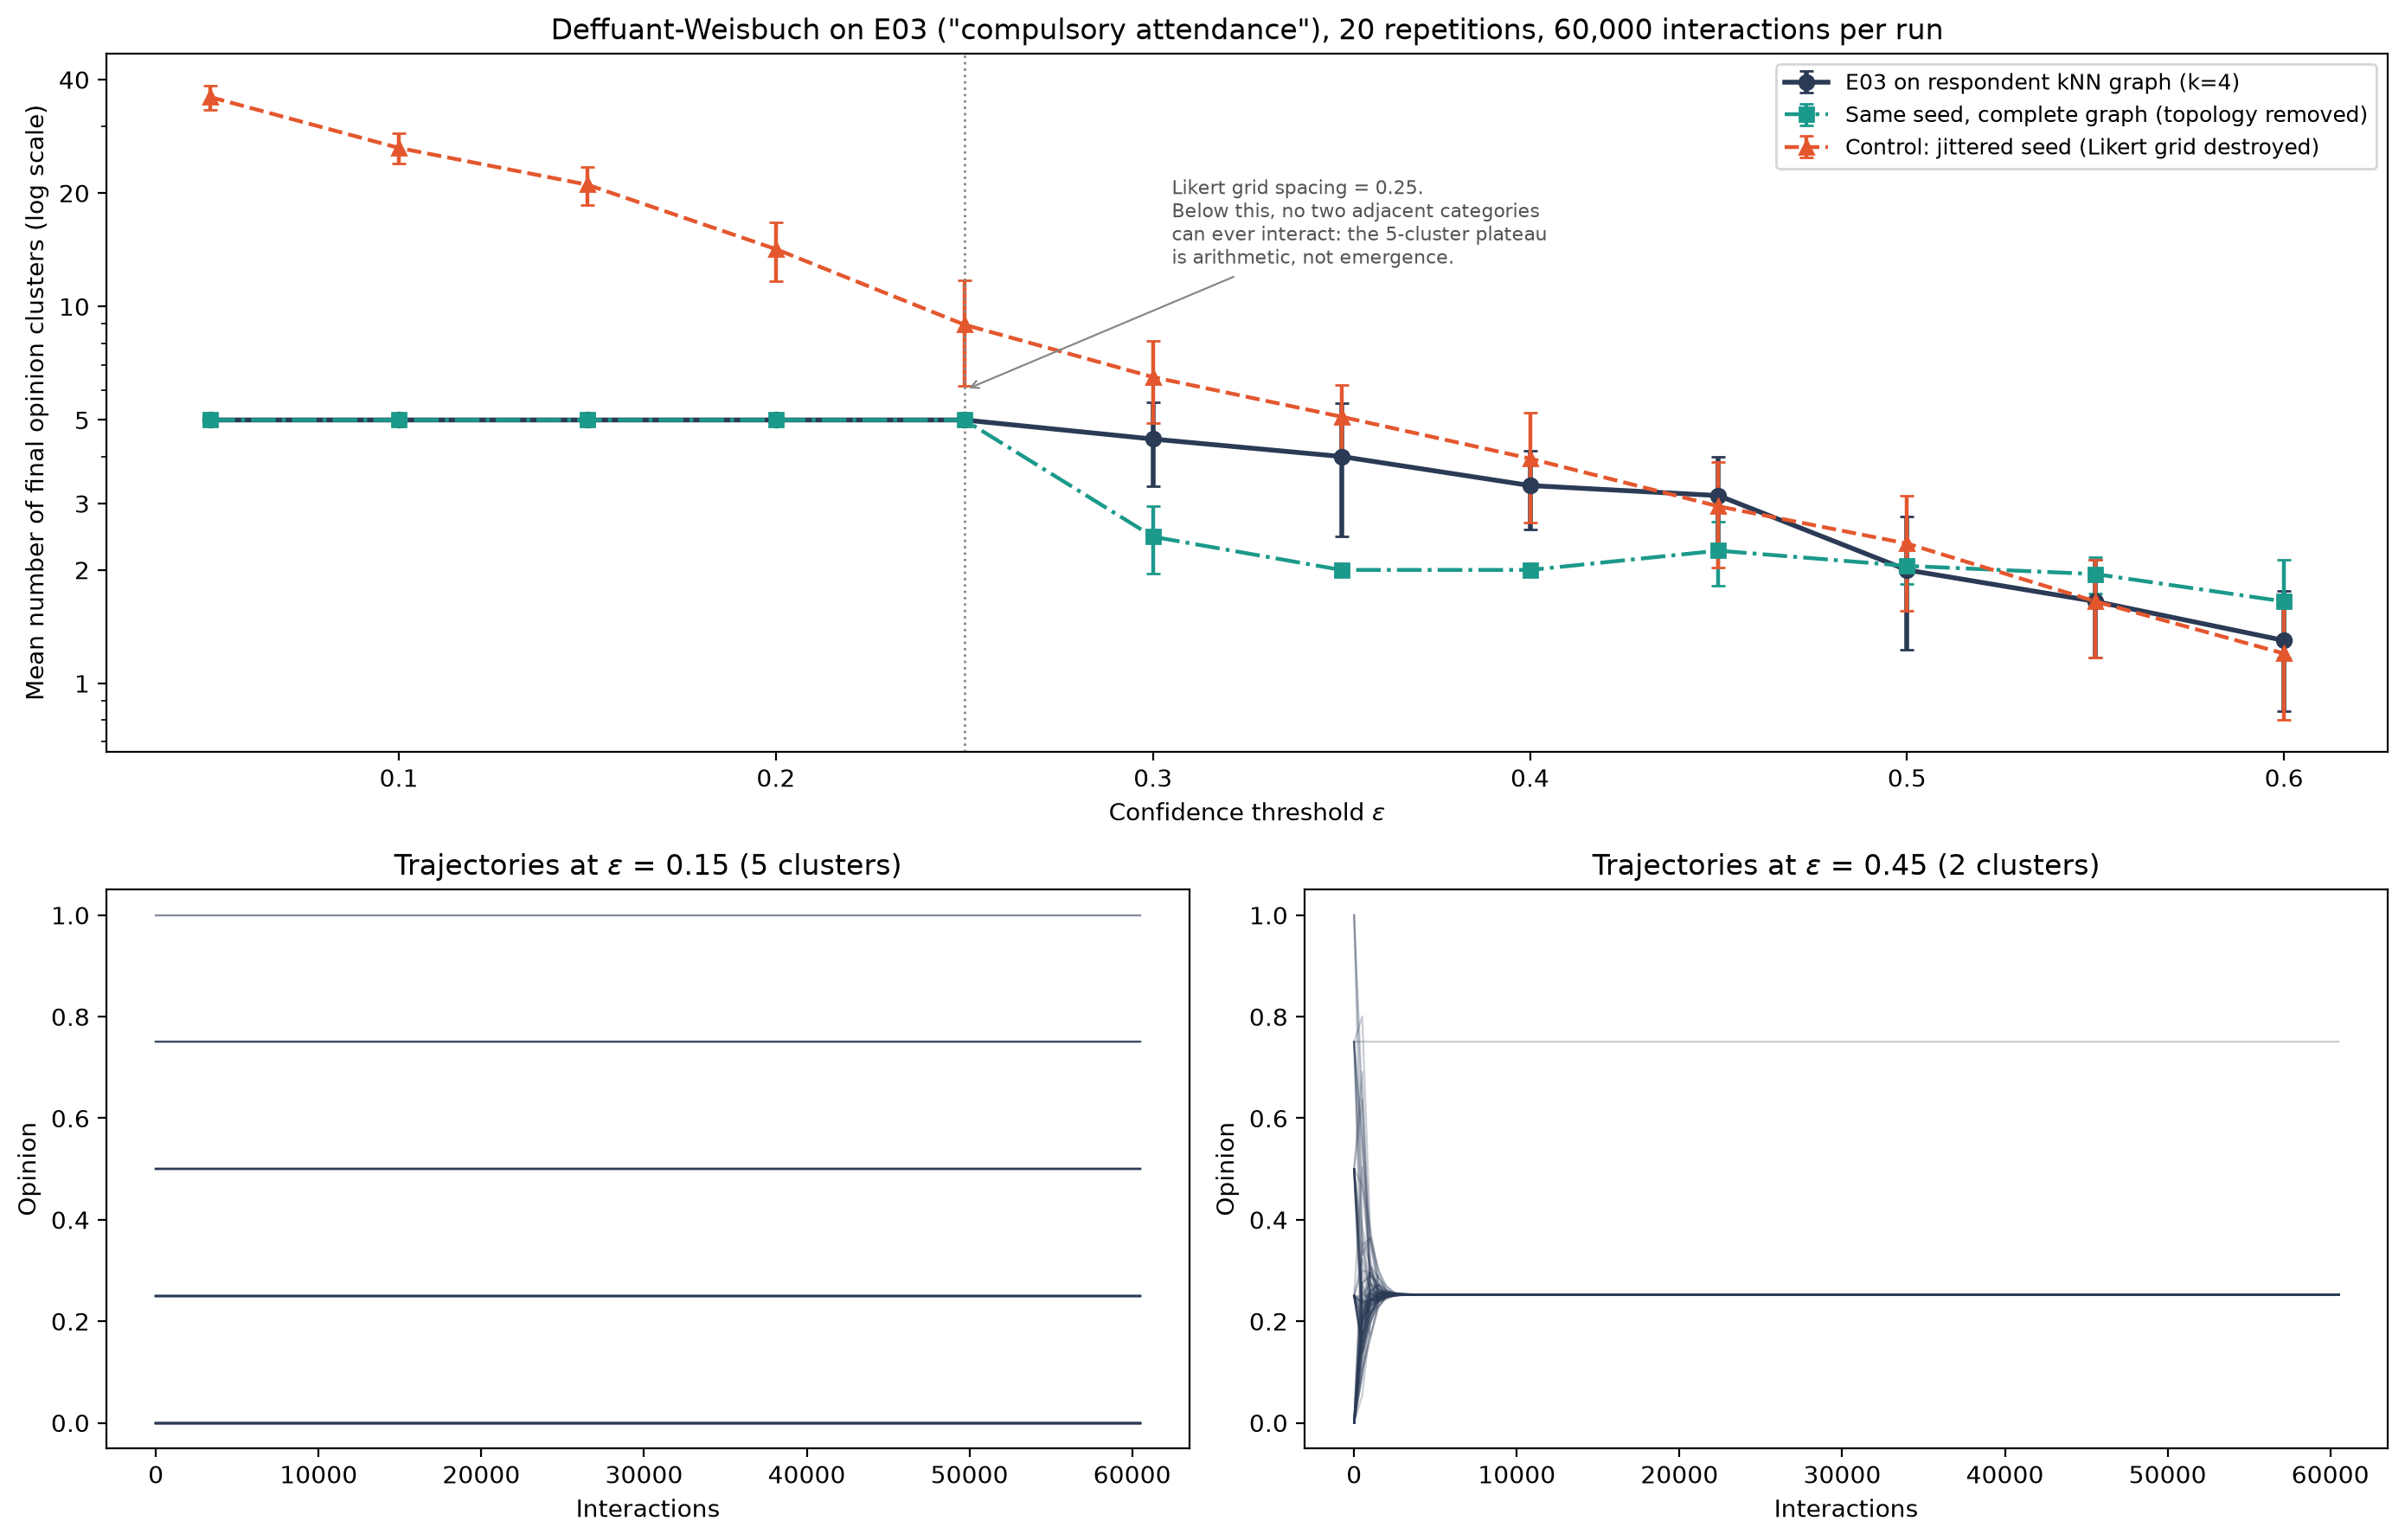
\includegraphics[width=0.84\textwidth]{../figures/graph12_deffuant_weisbuch.png}
\caption{Graph 12. Top: mean final cluster count against confidence threshold
$\varepsilon$ on a log scale, with error bars over 20 repetitions. The
$k$NN network and the complete graph coincide exactly below
$\varepsilon=0.25$---the signature of an arithmetic artefact---and diverge
above it, where topology matters. The jittered control destroys the response
grid and removes the plateau entirely. Bottom: individual opinion trajectories
at a low and a high $\varepsilon$, showing frozen categories against rapid
collapse.}
\label{fig:g12}
\end{figure*}

% ============================================================
\section{Results and Discussion}
\label{sec:discussion}
% ============================================================

\subsection{What the data supports}

\paragraph{Superficial consensus with genuine local structure.}
The headline finding is not polarisation. Agreement runs at $79.8\%$ across
every block and the leading principal component explains only about $8\%$ of
variance, so there is no evidence of two opposed camps. What exists instead is
a broad agreeable consensus with real but local disagreement concentrated in
specific, identifiable places.

\paragraph{Disagreement is domain-specific, not dispositional.}
Environment and society are effectively settled; technology and education are
not. Within education the cohort is precise about what it rejects---compulsory
attendance and written examinations---while endorsing curriculum reform and
problem-solving at above $94\%$. Within technology the objection tracks
delegated consequential judgment (medical diagnosis, autonomous vehicles)
rather than automation as such.

\paragraph{Most apparent structure was response style.}
Row-centring removes $87\%$ of the item pairs exceeding $|r|\geq0.30$. Any
analysis of this questionnaire that skips this step will find dense, uniformly
positive structure and will be measuring agreeableness.

\paragraph{Topology has a measurable dynamical consequence.}
In the bounded-confidence model, the sparse respondent network sustains
noticeably more opinion clusters than a well-mixed population at the same
tolerance, over the range where the dynamics are genuinely active.

\subsection{What the data does not support}

\todoblock{Results and Discussion --- integration, owner: P3}{%
Once Graphs 4--11 are complete, integrate their findings here. In particular
this section must state:\\[0.25em]
(i) whether the observed community structure survives the
\emph{permutation} null of Graph 10, and if it does not, report that the
communities are largely a construction artefact --- as a finding;\\[0.25em]
(ii) how many eigenvalue modes exceed the Marchenko--Pastur band (Graph 5) and
what fraction of variance is therefore attributable to signal rather than
noise;\\[0.25em]
(iii) whether the detected communities align with the four thematic blocks or
cut across them (Graphs 6 and 9);\\[0.25em]
(iv) whether structural balance strengthens with threshold (Graph 11).}

\subsection{Methods considered and rejected}

Documenting what did not work is part of the analysis. Four alternatives were
evaluated and set aside.

\textbf{Recoding NC as Neutral} imposes a systematic shift of about $0.92$
scale points at those cells and asserts a response that was explicitly
withheld. \textbf{Dropping NC users} removes roughly a fifth of the sample to
eliminate 37 cells and is the only NC treatment that substantially disturbs
the recovered partition (AMI $0.337$). \textbf{Excluding respondents by
missing-item count} was rejected because, once the five empty records are
removed, no substantial population of badly-incomplete respondents remains:
the rest are $95.6\%$ complete, and model-based recovery is preferable to
discarding usable respondents. \textbf{Mutual $k$NN} for the respondent
network fragments the graph into many components, which would inflate cluster
counts in the dynamics for reasons unrelated to the process being studied;
union $k$NN yields a single connected component.

\todoblock{Rejected methods --- additions from P2/P3}{%
Add the rejected sparsification and similarity variants once measured:
percentile thresholding at p90 (reported to leave $22$ components and many
isolates), cosine similarity and Gower distance as alternatives to Pearson,
and raw uncentred similarity (near-complete graph --- partially covered by
Graph 3).}

\subsection{Limitations}

Four limits bound every claim above. The response ceiling means items with
means above roughly $4.5$ measure social desirability more than preference
strength, and because few items are reverse-worded, acquiescence and a genuine
ceiling cannot be fully separated. The sample is $n=96$ from a single
institution, so differences of a few percentage points between statements are
noise and only the large gaps are safely above sampling variation. Dropout is
monotone, so later blocks rest on a slightly smaller base than earlier ones.
And the file carries no demographic fields, so no finding can be attributed to
any subgroup without additional joined data.

A methodological limitation deserves separate mention: correlation stability
under perturbation does not imply partition stability. Table~\ref{tab:sens}
shows correlation matrices agreeing at $r>0.94$ across NC treatments whose
community assignments agree at AMI $0.337$. Community-level conclusions
require their own stability analysis, by respondent-level bootstrap
resampling, before being treated as findings.

% ============================================================
\section{Conclusion}
\label{sec:conclusion}
% ============================================================

We presented an end-to-end pipeline from a raw ordinal questionnaire to an
opinion network and a dynamical process on it. Sanitisation preserves the
distinction between abandonment and deliberate non-response, retains all 91
non-empty respondents, and recovers $242$ missing cells by question-wise
regularised proportional-odds ordinal regression, which beats a modal baseline
under both scattered and structural artificial masking. Row-centring then
removes the acquiescence component that would otherwise dominate every
correlation, an intervention whose magnitude we quantify rather than assume:
it eliminates $87\%$ of item pairs correlated at $|r|\geq0.30$. On the
resulting matrix we build signed item and respondent networks and run
bounded-confidence dynamics, showing by direct argument and controlled
experiment that the small-$\varepsilon$ cluster plateau is forced by the
five-point response grid, while the diversity sustained by the sparse network
relative to a well-mixed population is a genuine topological effect.

\todoblock{Conclusion --- final integration}{%
Complete once Graphs 4--11 land. State the final chosen threshold and its
justification, the number of communities and whether they survive the
permutation null, and close on the overall characterisation of the cohort ---
superficial consensus with genuine local clustering --- supported by the
completed null-model evidence rather than asserted.}

% ============================================================
\section*{Individual Contribution}
% ============================================================

\begin{table}[h]
\caption{Contribution by team member.}
\vskip 0.05in
\begin{center}
\footnotesize
\begin{tabular}{p{0.16\columnwidth}p{0.70\columnwidth}}
\toprule
Member & Contribution \\
\midrule
Arijeet Paul &
Data sanitation and missingness analysis; ordinal-regression imputation and
its masking validation; row-centring; Graphs 1, 2, 3 and 12; respondent
$k$NN network; repository structure and \texttt{run\_all.py}. \\
\addlinespace
Shreyash Lohare & \textit{[TO BE COMPLETED --- Graphs 4, 5, 7]} \\
\addlinespace
Dev Patel & \textit{[TO BE COMPLETED --- Graphs 6, 10, 11]} \\
\bottomrule
\end{tabular}
\end{center}
\end{table}

\todoblock{Individual contribution}{%
Each member should replace their row with specific, auditable contributions
(modules written, figures produced, sections drafted). \texttt{git log}
provides the record.}

\bibliography{references}
% falls back to a standard style when icml2025.bst is absent
\IfFileExists{icml2025.bst}{\bibliographystyle{icml2025}}{\bibliographystyle{plain}}

\end{document}
